\refstepcounter{section}
\section*{Lecture 29: Stability Analysis}
\addcontentsline{toc}{section}{Lecture 29: Stability Analysis}
In the previous lecture, we saw a map over which we iterate our system to perform the decimation. This map resulted in two fixed points, $K^*=0$ and $K^*\to \infty$ for the 1D Ising model case. $K^*=0$ was a stable fixed point and hence starting the process from any $K\tund{0}>0$ resulted in convergence to zero, which denoted the infinite temperature, non-interacting case. \\[0.2cm]
Let us proceed to understand a general procedure to analyse the stability of these kind of maps. We will focus on the \textit{logistic map}, given by:
\begin{equation}\label{logistic}
    x_{n+1} = \mu x_n (1-x_n) \qquad x_n \in [0,1]
\end{equation}
Consider the function $f(x) =\mu x(1-x) = -\mu \qty[\qty(x-\frac{1}{2})^2-\frac{1}{4}]$. It has a maxima of $\frac{\mu}{4}$ at $x=\frac{1}{2}$. Hence, if $\mu>4$ then the maxima goes beyond $1$ and then Eq. \eqref{logistic} no longer maps $[0,1]$ to itself. And we should always be positive. Hence, we keep the control parameter $0< \mu \leq 4$.\\[0.2cm]
Let us now calculate the fixed points. Let $x^*$ be the fixed point which implies, 
\begin{align}
    \begin{split}
        f(x^*) = x^* \implies \mu x^* (1-x^*) = x^* \implies x^* = 0 \quad \text{or } \quad x^* = 1-\frac{1}{\mu}
    \end{split}
\end{align} 
Now, we calculate the stability of these fixed points. ``Stability'' refers to the situation that if we start at some point around $x^*$, then do we fall into $x^*$ or go away from $x^*$. For this, consider a sequence $\epsilon_n$ such that, 
$$x_n = x^* + \epsilon_n$$
Then, the fixed point condition $x^* = f(x^*)$ gives us,
\begin{align*}
  x^*+\epsilon_{n+1} = x_{n+1} = f(x_n) = f(x^*+\epsilon_n) \xrightarrow{Taylor} f(x^*) + \epsilon_n f'(x^*) =  x^* +  \epsilon_n f'(x^*)
\end{align*}
The above condition implies $\abs{f'(x^*) }=\abs{ \frac{\epsilon_{n+1}}{\epsilon_n}}$ and this tells us a lot. From the map, we have $f'(x^*) = mu (1-2x^*)$. For $x^*=0$ we have $f'(0) = \mu$ and for $x^*=1-\frac{1}{\mu}$ we have $f'(x^*)=2-\mu$. For stability, we need the sequence $\{\abs{\epsilon_n}\}$ to be decreasing, that is, $|\epsilon_{n+1}|<|\epsilon_n| \implies |f'(x^*)|<1$. \\[0.2cm]
\triangleright\hspace{0.2cm} \textbf{Stability of $\boldsymbol{x^*=0}$}\\[0.2cm]
If $\abs{f'(0)} =\abs{ \mu} <1$ then $x^*=0$ is a stable fixed point. Thus, for $0<\mu<1$ we have $x^*=0$ is a \textit{stable point} of the map. This means that starting from any value of $x\tund{0}$, we will eventually converge to 0. \\[0.2cm]
\triangleright\hspace{0.2cm} \textbf{Stability of $\boldsymbol{x^*=1-\frac{1}{\mu}}$}\\[0.2cm]
If $\abs{f'(x^*)} =\abs{ 2-\mu} <1$ then $x^*=0$ is a stable fixed point. The condition leads to,
$$-1 < 2-\mu <1 \implies -3 <-\mu<-1\implies  1<\mu <3$$
Thus, for $1<\mu<3$ we have $x^*=1-\frac{1}{\mu}$ is a \textit{stable point} of the map. This means that starting from any value of $x\tund{0}$, we will eventually converge to $1-\frac{1}{\mu}$. Note that the point of convergence will now depend on the value of $\mu$.\\[0.2cm]
Beyond $mu=3$, none of the fixed points are stable and there are some other complicated things like period-doubling and chaos going on. It can be shown that for $3<r<1+\sqrt{6}$, there is a stable \textit{period-2 orbit}, which means that instead of $f(x^*) = x^*$ we have $f(f(x^*))=x^*$.\\[0.2cm]
Similarly for $1+\sqrt{6}<\mu<3.54409\ldots$ we have a \textit{period-4 orbit}. This way, period-$2^n$ occurs for different $\mu_n$ ($\mu_n$ is the value where the first bifurcation occurs). Successive bifurcations come faster and faster and ultimately $\mu_n$ converges to $\mu_\infty$ ($\approx 3.569946$ for the logistic map). For $\mu>\mu_\infty$, the dynamics become \textit{chaotic}.\\[0.2cm] These behaviour can be demonstrated using the \textit{orbit diagram}, generated numerically. What we do is, we choose a particular value of $\mu$ and then, choosing some initial value, we iterate the map for quite some generations (to kill of the initial transient behaviour). Then, we plot $x_n$ for multiple successive iterations. 
\begin{figure}[H]
    \centering
    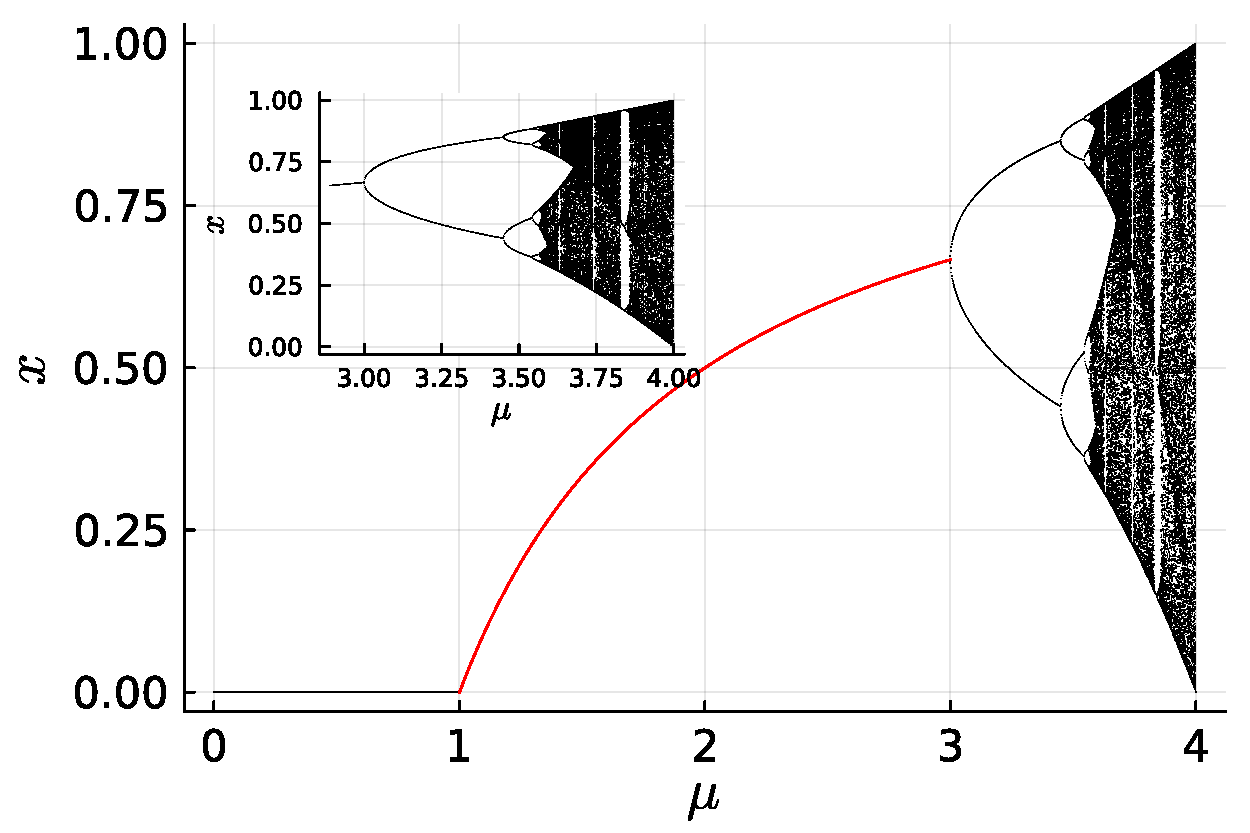
\includegraphics[width=0.7\textwidth]{codes/logistic_orbit.pdf}
    \caption{\textbf{Orbit diagram for logistic map.} We see that at $\mu=1$, there is a bifurcation. At $\mu=3$, there is another bifurcation (period doubling) and so on. The inset shows a zoomed in region between $3<\mu<4$ which shows further bifurcations. The red line shows the $x=1-\frac{1}{\mu}$ line. }
\end{figure}
Now, finally let us plot the cobweb diagrams for different values of $r$ which will make the case a bit more clear. 
\begin{figure}[H]
    \centering
    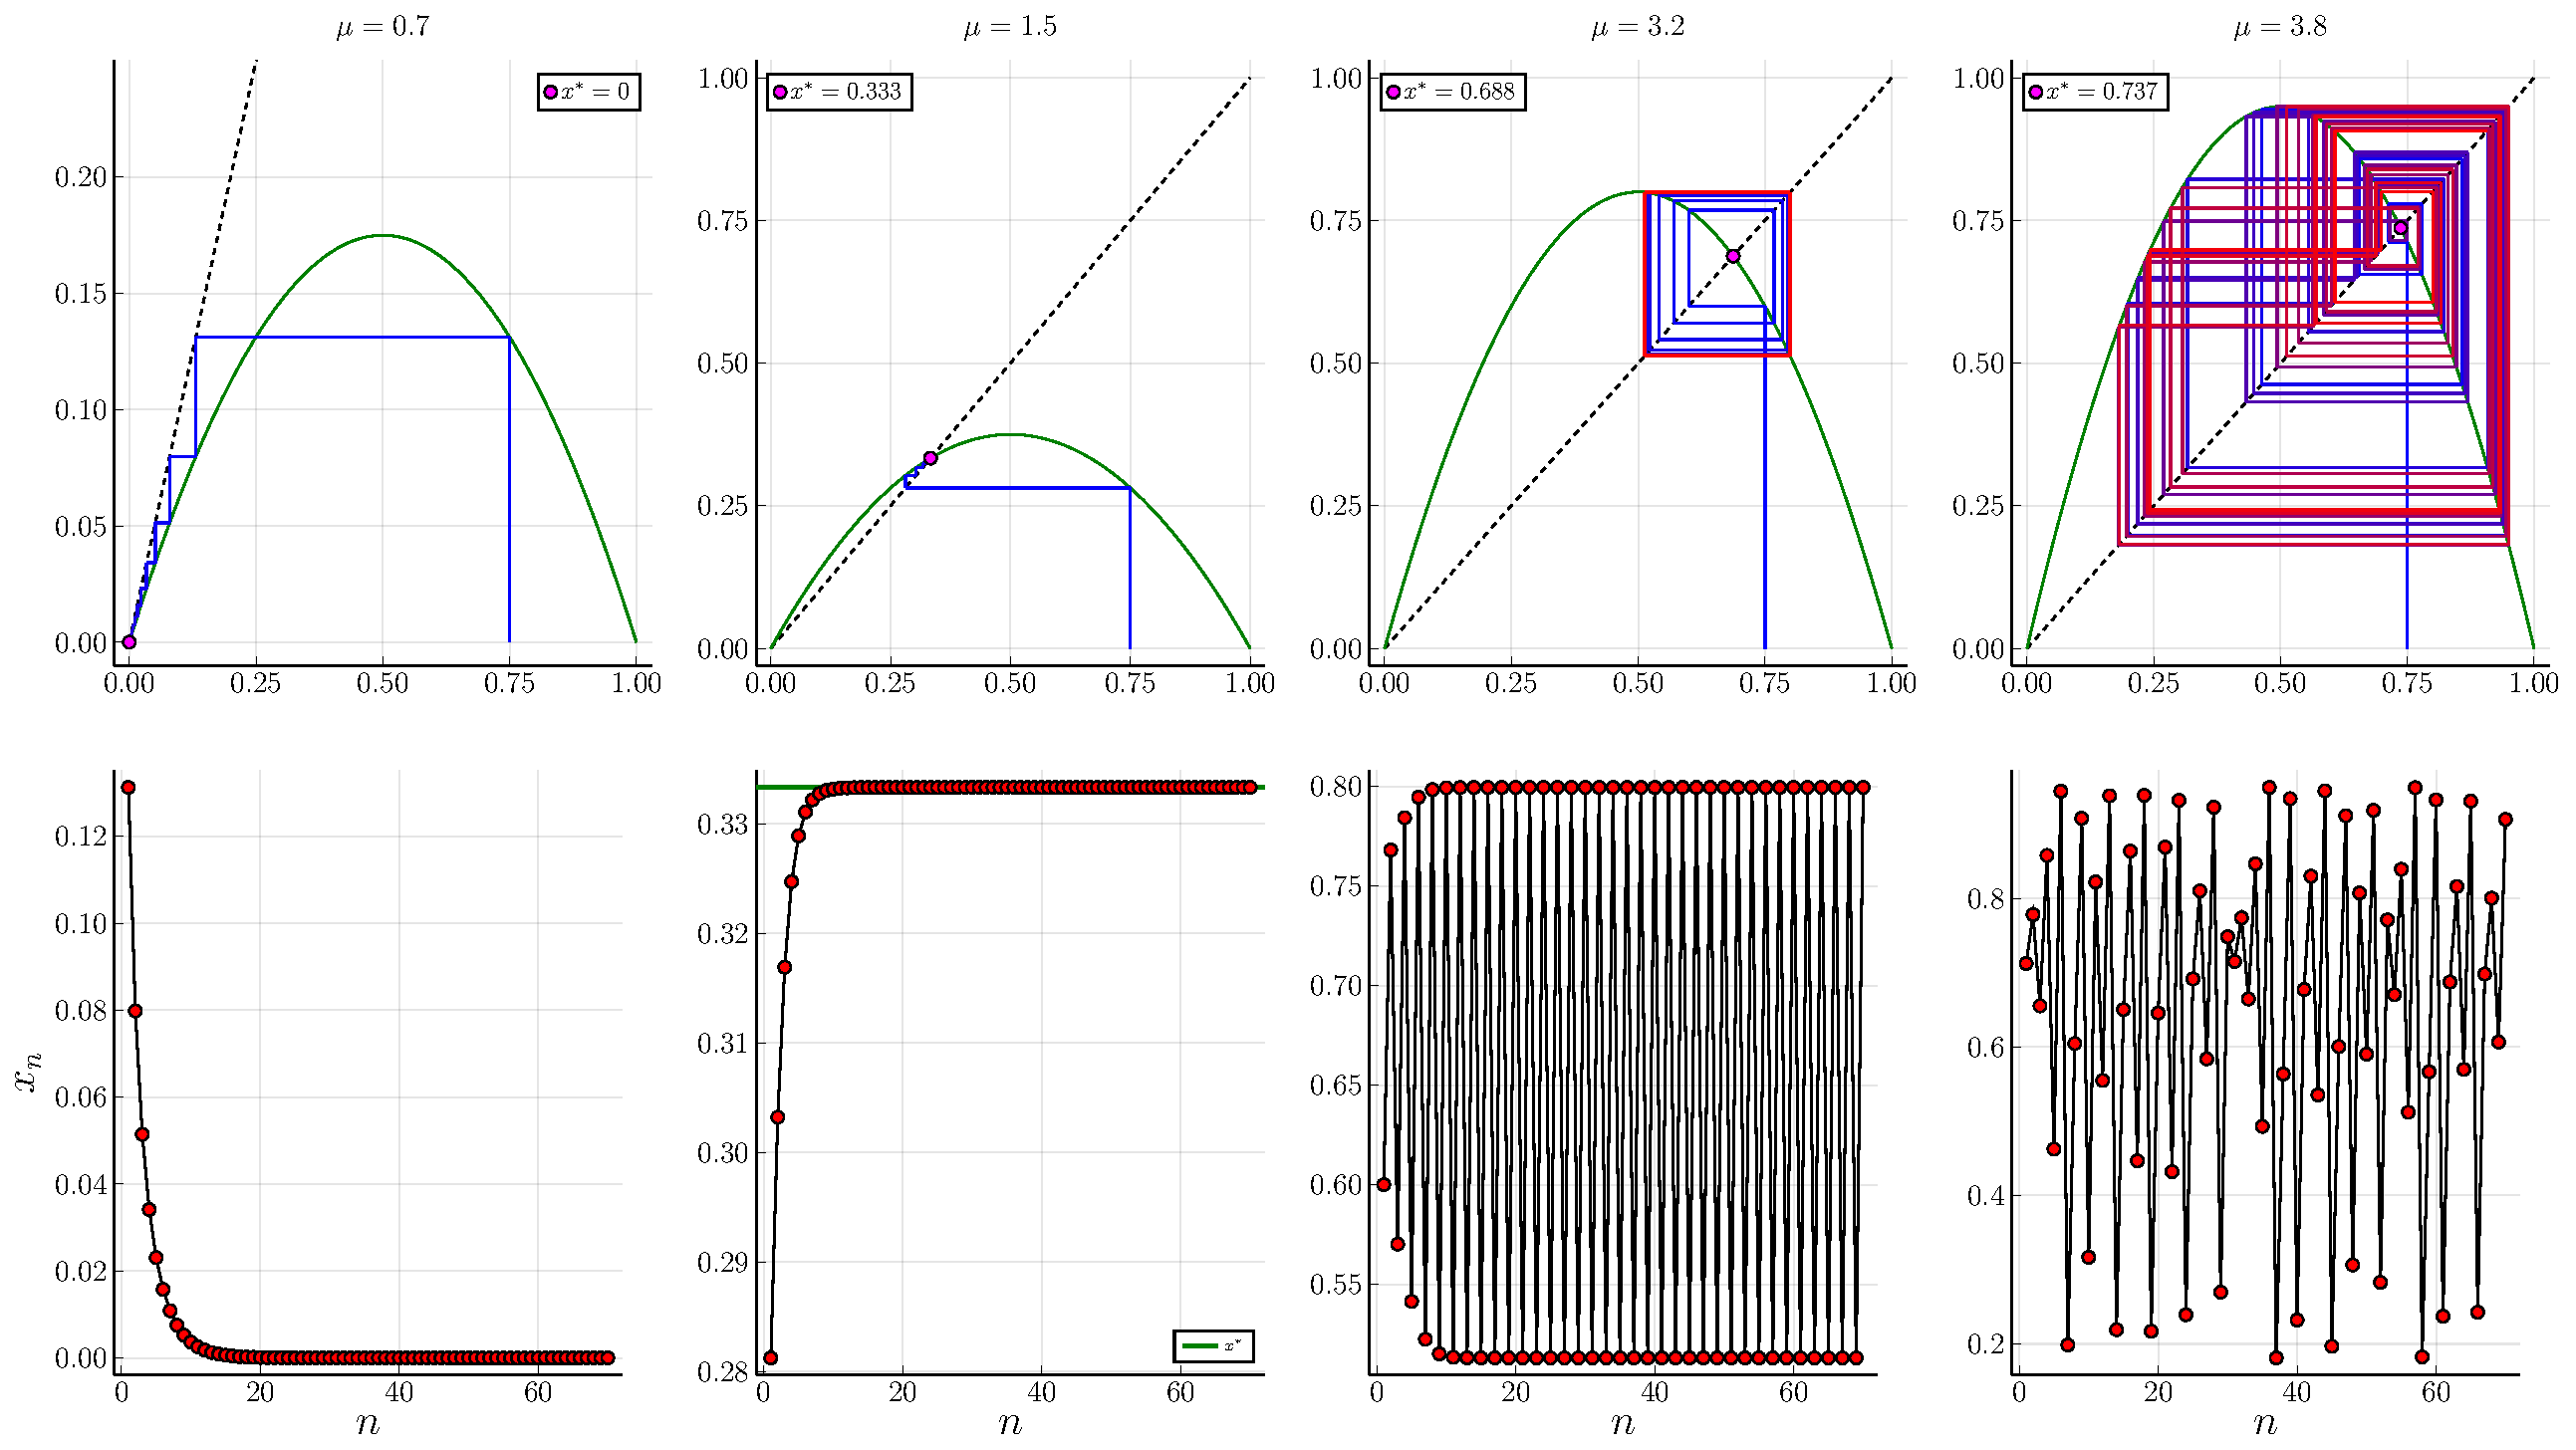
\includegraphics[width=\textwidth]{codes/timewaste.pdf}
    \caption{\textbf{Cobweb diagram for different $\boldsymbol{\mu}$.} The upper panel shows the cobweb diagram of the logistic map for different values of $\mu$ while the lower panel shows the corresponding convergence of the map under successive iterations. For the third panel, there is no convergence but there is a periodic orbit with period 2 and in the last panel, there is no pattern as such, the evolution is \textit{chaotic}. }
\end{figure}